\cmfnewsection{Introdução}{./logos/fundo_tese}{0.15}




%
%
%%%%%%%%%%%%%%%%%%%%%%%%%%%%%%%%%%%%%%%%%%%%%%%%%%%%%%%%
%%%%%%%%%%%%%%%%%%%%%%%%%%%%%%%%%%%%%%%%%%%%%%%%%%%%%%%%
%%%%%%%%%%%%%%%%%%%%%%%%%%%%%%%%%%%%%%%%%%%%%%%%%%%%%%%%
%\begin{frame}{Conversores Fonte de Tensão}
%
%
%\begin{columns}
%
%\column{0.5\linewidth}
%\centering
%Conversor de dois níveis
%\vspace*{0.5cm}
%
%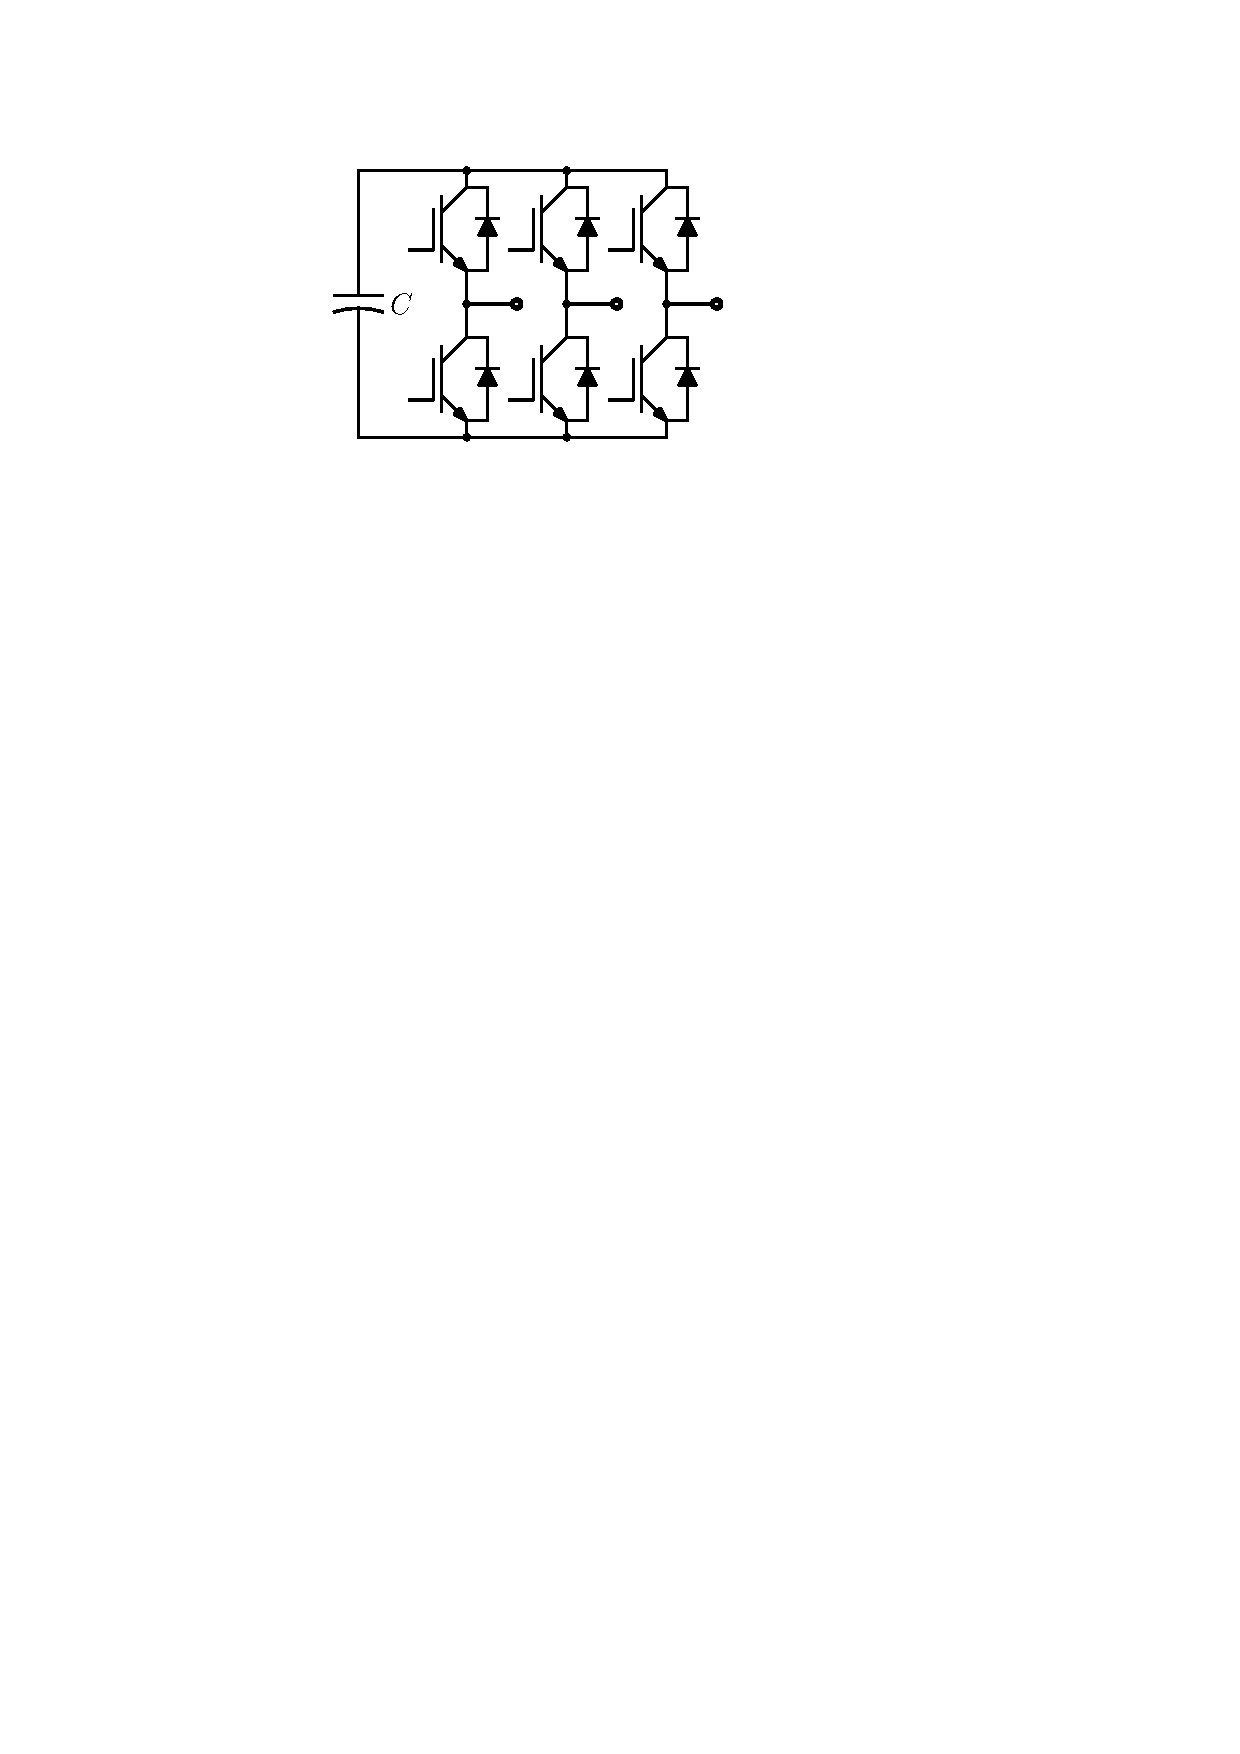
\includegraphics[width=0.8\linewidth]{./figuras/introducao/2niveis}
%
%
%\column{0.5\linewidth}
%
%\begin{itemize}
%	\item Baseados em IGBT\\[15pt]
%	\item Alta frequência de comutação\\[15pt]
%	\item Totalmente controlável\\[15pt]
%	\item Comum na industria\\[15pt]
%	\item {\color{red}Filtros (dependendo da aplicação)}\\[15pt]
%	\item {\color{red}Limitações em alta tensão}
%\end{itemize}
%
%
%
%
%\end{columns}
%
%
%
%
%
%\end{frame}





%%%%%%%%%%%%%%%%%%%%%%%%%%%%%%%%%%%%%%%%%%%%%%%%%%%%%%%
%%%%%%%%%%%%%%%%%%%%%%%%%%%%%%%%%%%%%%%%%%%%%%%%%%%%%%%
%%%%%%%%%%%%%%%%%%%%%%%%%%%%%%%%%%%%%%%%%%%%%%%%%%%%%%%
\begin{frame}{Conversores Fonte de Tensão: Dois Níveis}


\begin{columns}

\column{0.5\linewidth}
\centering

Baixa Tensão\\[20pt]

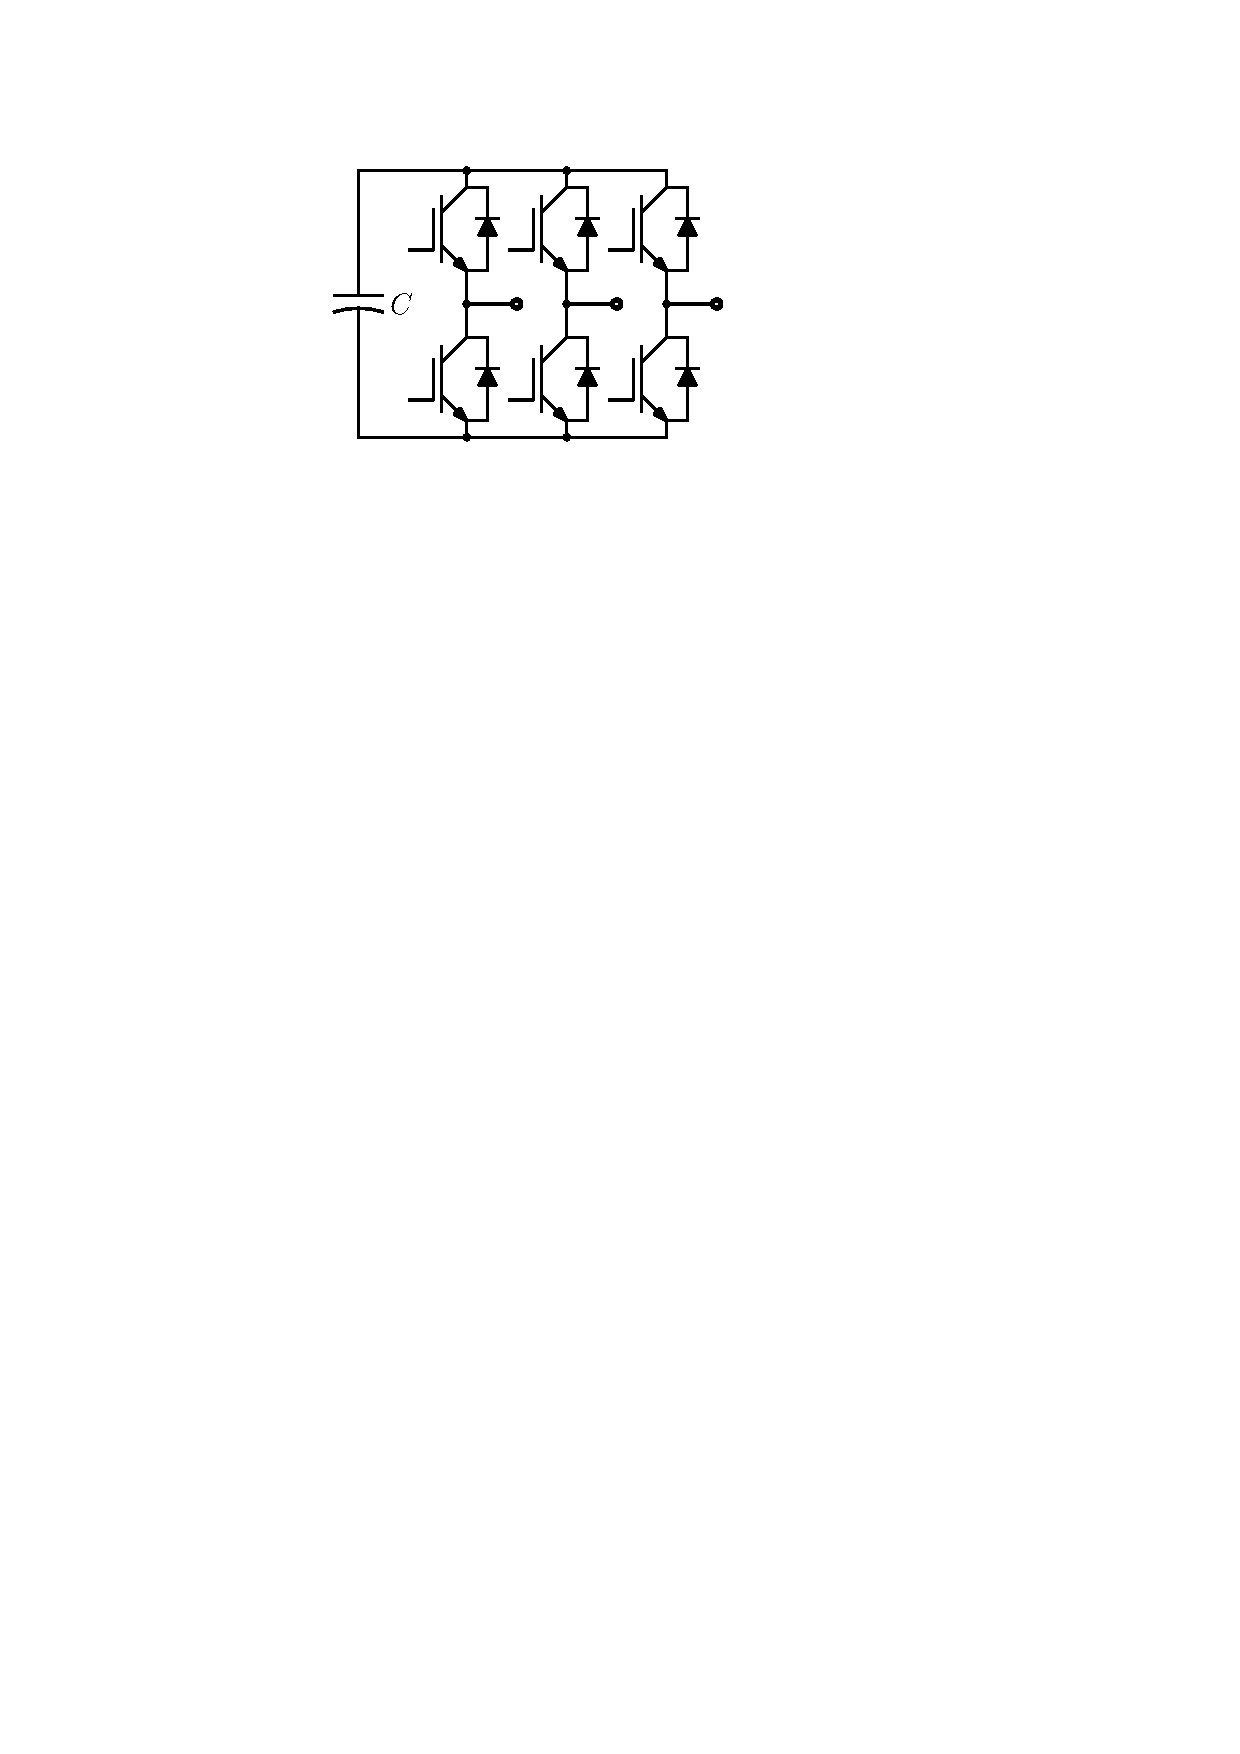
\includegraphics[width=0.6\linewidth]{./figuras/introducao/2niveis}


\column{0.5\linewidth}
\centering


Média e Alta Tensão\\[20pt]

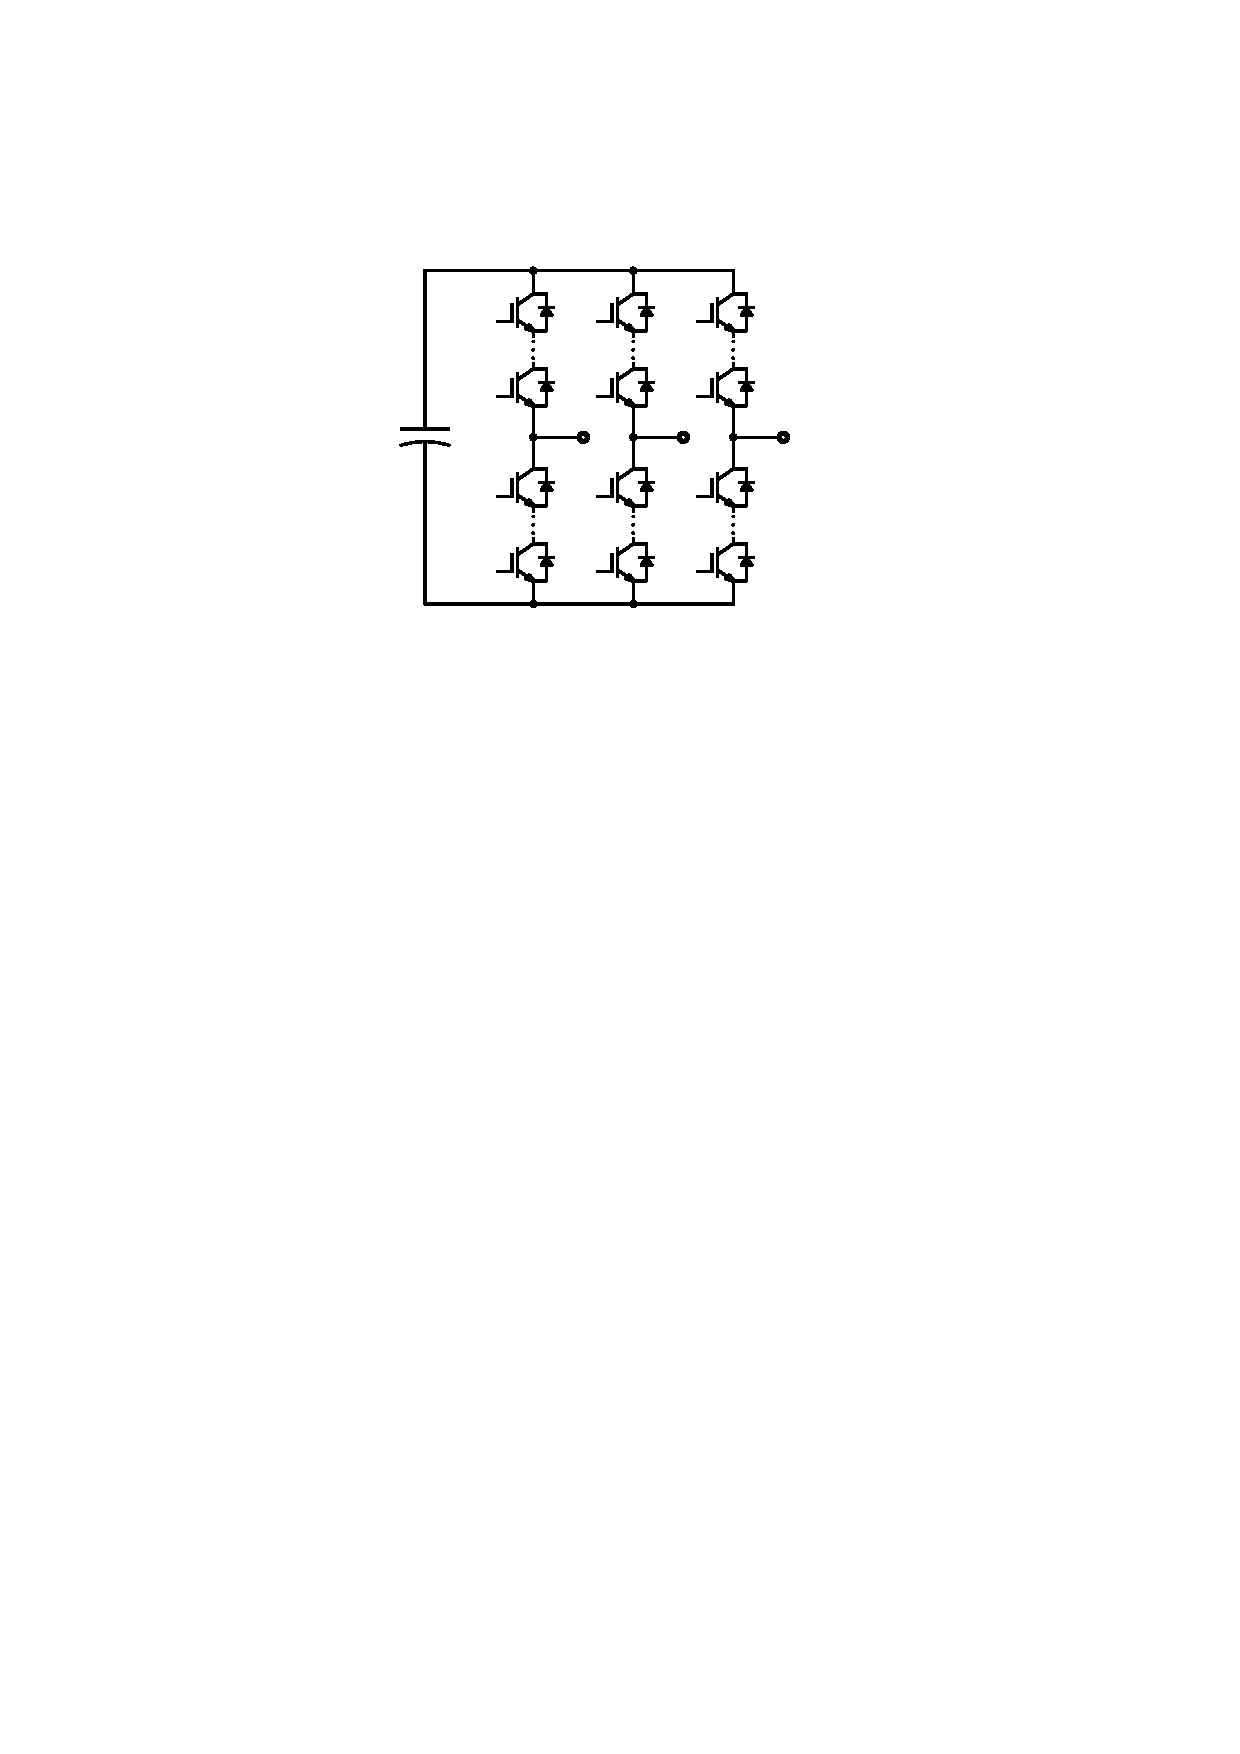
\includegraphics[width=0.55\linewidth]{./figuras/introducao/2niveis_alta}



\end{columns}





\end{frame}



%%%%%%%%%%%%%%%%%%%%%%%%%%%%%%%%%%%%%%%%%%%%%%%%%%%%%%%
%%%%%%%%%%%%%%%%%%%%%%%%%%%%%%%%%%%%%%%%%%%%%%%%%%%%%%%
%%%%%%%%%%%%%%%%%%%%%%%%%%%%%%%%%%%%%%%%%%%%%%%%%%%%%%%
\begin{frame}{Conversor Multinível Modular (MMC)}



\begin{columns}

\column{0.5\textwidth}



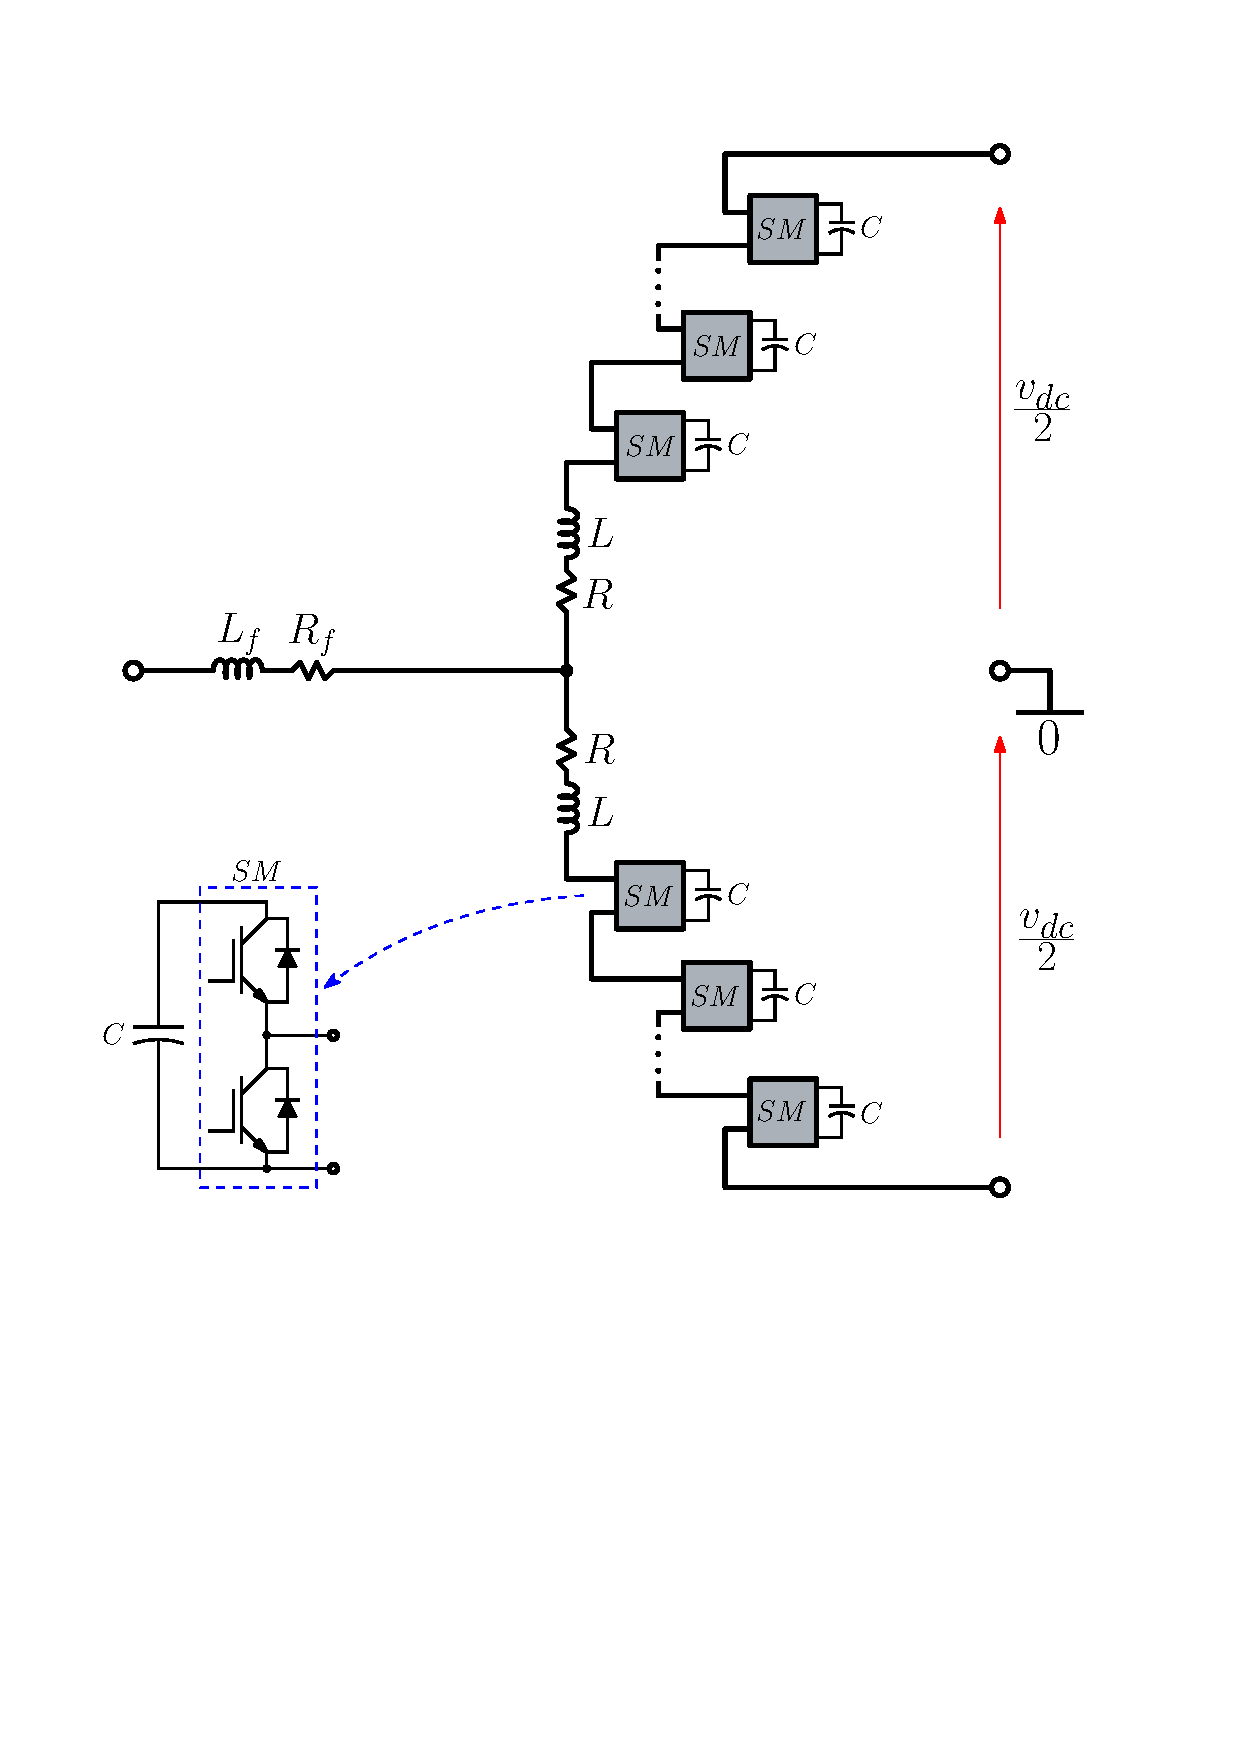
\includegraphics[width=0.9\linewidth]{./figuras/introducao/MMC_blk_limpo}







\column{0.5\textwidth}

%Aplicações

\definecolor{heavy-gray}{rgb}{0.31,0.31,0.31}




\begin{itemize}
	\item Associação de vários submódulos \\[25pt]
	\item Aplicações em alta tensão \\[25pt]
	\item Facilmente escalonável \\[25pt]
	\item {\color{blue}HVDC} \\[25pt]
	\item {\color{blue}FACTs}
\end{itemize}



\end{columns}



\end{frame}









%%%%%%%%%%%%%%%%%%%%%%%%%%%%%%%%%%%%%%%%%%%%%%%%%%%%%%%
%%%%%%%%%%%%%%%%%%%%%%%%%%%%%%%%%%%%%%%%%%%%%%%%%%%%%%%
%%%%%%%%%%%%%%%%%%%%%%%%%%%%%%%%%%%%%%%%%%%%%%%%%%%%%%%
\begin{frame}{Atualidade: Conexão de Usinas Eólicas {\it Offshore}}

\centering

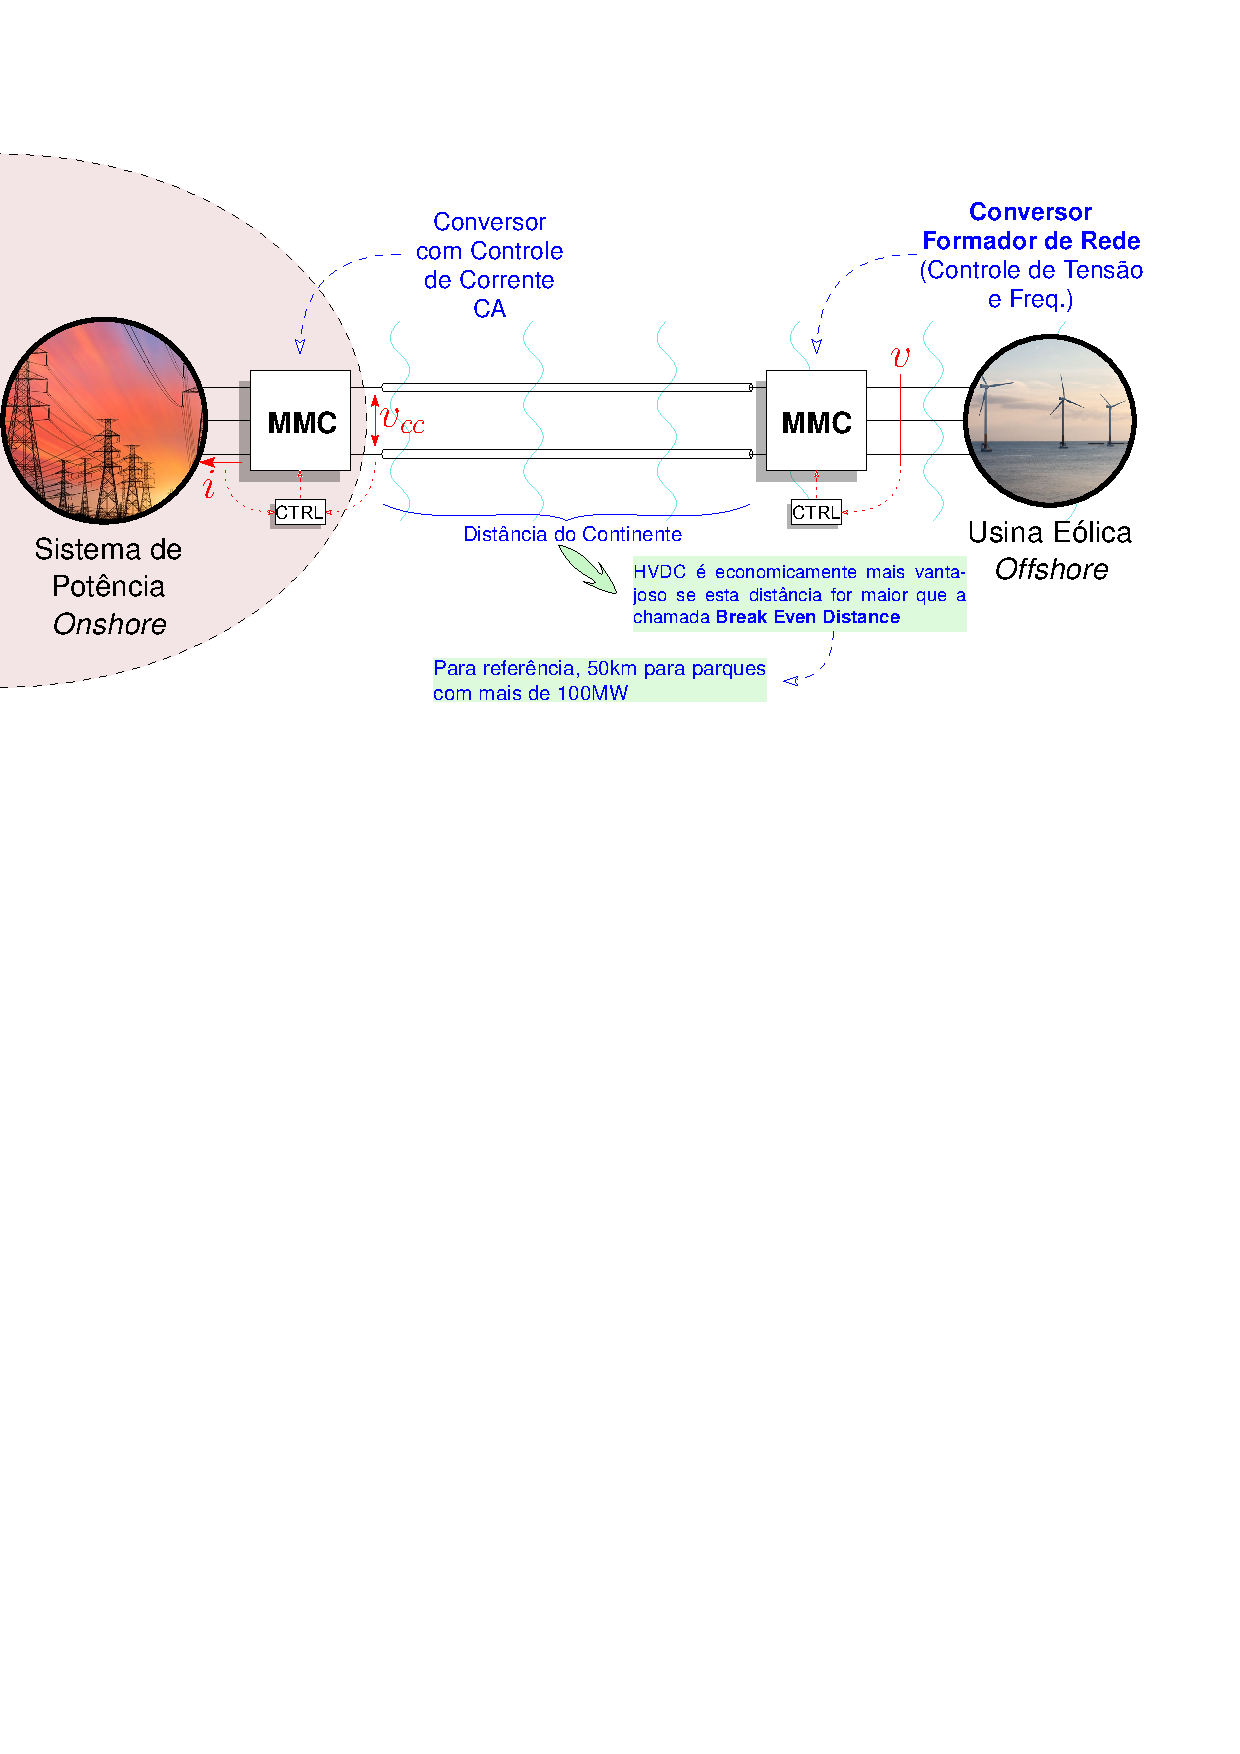
\includegraphics[width=\linewidth]{./figuras/introducao/MMC-HVDC-2}


\end{frame}











%%%%%%%%%%%%%%%%%%%%%%%%%%%%%%%%%%%%%%%%%%%%%%%%%%%%%%%
%%%%%%%%%%%%%%%%%%%%%%%%%%%%%%%%%%%%%%%%%%%%%%%%%%%%%%%
%%%%%%%%%%%%%%%%%%%%%%%%%%%%%%%%%%%%%%%%%%%%%%%%%%%%%%%
\begin{frame}{Foco do Trabalho}



\begin{itemize}
	\item Obter modelos matemáticos analíticos no domínio da frequência considerando diferentes modos de controle: 
	
	\begin{itemize}
		\item Controle por corrente CA
		\item Controle por tensão CA (formador de rede)
		\item Controle em referencial natural
		\item Controle em referencial síncrono
	\end{itemize}

	\item Realizar análises:
	
	\begin{itemize}
		\item Influência dos controladores
		\item Derivações de impedâncias/admitâncias virtuais para melhorar a performance do MMC
	\end{itemize}
	
	\item Apresentar aplicação:
	
	\begin{itemize}
		\item Análise de estabilidade de sistemas baseados em MMC
	\end{itemize}
	
	
\end{itemize}










%Modelos em referencial natural e em referencial síncrono para o MMC formador de rede com malha dupla (corrente e tensão).


%
%\begin{itemize}
%	\item Será focada nos modelos ;
%	
%	\item Considerar um banco capacitivo $C_f$ (...)
%	
%	\item Obter o modelo para a malha de corrente
%	
%	\item Obter um modelo para malha de tensão sem considerar $C_f$
%	
%	\item Incluir $C_f$ no modelo.
%\end{itemize}


\end{frame}





